\selectlanguage{ngerman}%
\frenchspacing%
\begin{ledgroupsized}[r]{120mm}%
\footnotesize%
\pstart%
\noindent%
\textbf{Überlieferung:}%
\pend%
\end{ledgroupsized}%
\begin{ledgroupsized}[r]{114mm}%
\footnotesize%
\pstart%
\parindent -6mm%
\makebox[6mm][l]{\textit{L}}%
Notiz:
LH XXXVIII Bl.\;157.
Ein Zettel;
Ränder beschnitten.
Eine Seite auf Bl.\;\href{\Scan{LH_38_157r}}{157\,r\textsuperscript{o}}.
Bl.\;\href{\Scan{LH_38_157v}}{157\,v\textsuperscript{o}} ist unbeschrieben.
\pend%
\end{ledgroupsized}%
\vspace{5mm}%
\begin{ledgroup}%
\footnotesize%
\pstart%
\noindent%
\textbf{Datierungsgründe:}
Die Datierung der Aufzeichnung N.\;\ref{55805} beruht auf %
inhaltlichen Betrachtungen.
Siehe die ausführliche Begründung auf S.\;\pageref{55805_dat}.%
\pend%
\end{ledgroup}%
\selectlanguage{latin}%
\frenchspacing%
\vspace*{8mm}
\normalsize%
\pstart%
\noindent%
\lbrack%
\href{\Scan{LH_38_157r}}%
{157\,r\textsuperscript{o}}%
\rbrack\
Quaeritur
an majori fructu%
\indexS{fructus}
aer externus impellatur%
\indexS{aer externus}%
\indexS{aer impulsus}
immediata eruptione aeris compressi,%
\indexS{aer compressus}%
\indexS{eruptio aeris compressi}
an alis actis.%
\indexS{ala}
Et videntur alae praestare
ob aeris divisibilitatem.%
\indexS{divisibilitas aeris}
Ponantur jactus%
\indexS{jactus aquae}
\edtext{%
aquae\;\textit{AB}%
\indexS{aqua jacta}
emissi in alam\;\textit{C}
ex corpore\;\textit{D}%
}{%
\lemma{aquae}%
\Bfootnote{%
\bars{\textit{AB} \textit{erg.}} emissi %
\textit{(1)}~ex corpore %
\textit{(2)}~in %
\textit{(a)}~corpus %
\textit{(b)}~alam \textit{C}, ex corpore \textit{D}%
~\textit{L}%
}}
aerem impellere%
\indexS{aer impulsus}
ope alae,%
\indexS{ala}
\edtext{%
quaeritur
an corpus\;\textit{D} fortius hoc remigio%
\indexS{remigium}%
}{%
\lemma{quaeritur}%
\Bfootnote{%
\textit{(1)}~an corpus \textit{D} hoc %
\textit{(2)}~an aer %
\textit{(3)}~an corpus \textit{D} %
\textit{(a)}~hoc modo %
\textit{(b)}~fortius hoc remigio%
~\textit{L}%
}}
impellatur,
quam si jactus illi%
\indexS{jactus aquae}
simpliciter in aerem agerent%
\lbrack;\rbrack\
ita arbitror,
aer%
\indexS{aer excipiens motum}%
\indexS{aer sistens motum}
\edtext{%
enim non totum jactus motum
excipit sistitque,
sed dividens sese%
\indexS{aer dividens se}
transitum ei permittit.%
\indexS{transitus in aere}%
}{%
\lemma{enim}%
\Bfootnote{%
\textit{(1)}~dividens sese %
\textit{(2)}~non totu %
\textit{(3)}~\bars{non \textit{erg.}} totum jactus motum %
\textit{(a)}~accipit %
\textit{(b)}~excipit sistitque, %
\lbrack...\rbrack\ ei permittit.%
~\textit{L}%
}}
Idem ergo de jactibus aeris%
\indexS{jactus aeris}%
\indexS{aer jactus}
dicendum esse patet.
\pend%
\begin{edfigure}[2.75em][0.0em]%
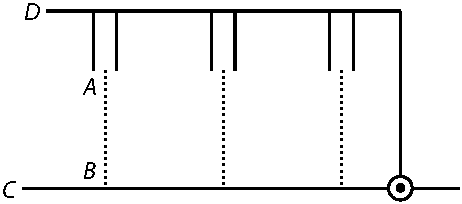
\includegraphics[width=0.48\textwidth]{gesamttex/edit_VIII-4/images/LH_38_04_157-d_157r.pdf}
\edcaption[1.0em]%
{%
\lbrack\textit{Fig.\:1}\rbrack%
}%
\end{edfigure}%
\newpage%
\vspace{3.0em}%
\pstart%
\noindent%
\centering%
*     *     *
\pend%
\vspace{2.5em}%
\selectlanguage{german}%
\frenchspacing%
\footnotesize%
\pstart%
\noindent%
\textls{Ausführliche Datierungsgründe:}%
\pagelabel{55805_dat}
Die undatierte Notiz N.\;\ref{55805} setzt sich kurz mit der Frage auseinander, ob eine Luftmasse wirksamer von einem unmittelbaren Ausbruch zusammengedrückter Luft angestoßen werde oder aber durch die Vermittlung eines Flügels.
Leibniz nimmt für die zweite Alternative Stellung und begründet das mit Hinweis auf die Teilbarkeit der Luft.
Diese Überlegung könnte im Zusammenhang mit der von Leibniz eigenhändig auf Juni 1678 datierten Aufzeichnung N.\;\ref{55774} entstanden sein, in welcher der Gedanke ausgeführt wird, dass winzige Strahlen zusammengedruckter Luft ein angemessenes Mittel sein könnten, um die Flügel einer künstlichen Taube zu bewegen.
Unter Berücksichtigung dieser inhaltlichen Verwandtschaft erweist sich als plausibel, dass auch die Notiz N.\;\ref{55805} im Juni 1678 entstand.
Eine frühere oder eine spätere Datierung ist dennoch möglich.
Der Textträger (Bl.\;\href{\Scan{LH_38_157wz}}{157}) weist weder Spuren eines Wasserzeichens noch weitere datierungsrelevante Eigenschaften auf.
\pend%
\selectlanguage{latin}%
\frenchspacing%
\normalsize%
\newpage%
